%%%%%%%%%%%%
%% Please rename this main.tex file and the output PDF to
%% [lastname_firstname_graduationyear]
%% before submission.
%%
%% This .tex file is for use with BibLaTeX. Please use
%% main-bibtex.tex instead if you prefer BibTeX.
%%%%%%%%%%%%

\documentclass[12pt]{caltech_thesis}
\usepackage[hyphens]{url}
\usepackage{lipsum}
\usepackage{graphicx}

\usepackage{todonotes}
\usepackage{physics}

%% Tentative: newtx for better-looking Times
\usepackage[utf8]{inputenc}
\usepackage[T1]{fontenc}
\usepackage{newtxtext,newtxmath}

% Must use biblatex to produce the Published Contents and Contributions, per-chapter bibliography (if desired), etc.
\usepackage[
    backend=biber,natbib,
    % IMPORTANT: load a style suitable for your discipline
    style=chem-acs
]{biblatex}
\usepackage{nomencl}


\makenomenclature
%% This code creates the groups
% -----------------------------------------
\usepackage{etoolbox}
\renewcommand\nomgroup[1]{%
  \item[\bfseries
  \ifstrequal{#1}{M}{Molecular orbital basis}{%
  \ifstrequal{#1}{N}{Number sets}{%
  \ifstrequal{#1}{O}{Other symbols}{}}}%
]}
% -----------------------------------------

\usepackage{listings} % Required for insertion of code
\usepackage{xcolor} % Required for custom colors

% Define custom colors
\definecolor{codegreen}{rgb}{0,0.6,0}
\definecolor{codegray}{rgb}{0.5,0.5,0.5}
\definecolor{codepurple}{rgb}{0.58,0,0.82}
\definecolor{backcolour}{rgb}{0.95,0.95,0.92}

% Setup the style for code listings
\lstdefinestyle{mystyle}{
    backgroundcolor=\color{backcolour},   
    commentstyle=\color{codegreen},
    keywordstyle=\color{magenta},
    numberstyle=\tiny\color{codegray},
    stringstyle=\color{codepurple},
    basicstyle=\ttfamily\footnotesize,
    breakatwhitespace=false,         
    breaklines=true,                 
    captionpos=b,                    
    keepspaces=true,                 
    numbers=left,                    
    numbersep=5pt,                  
    showspaces=false,                
    showstringspaces=false,
    showtabs=false,                  
    tabsize=2
}

% Activate the style
\lstset{style=mystyle}


% Name of your .bib file(s)
\addbibresource{examples.bib}
\addbibresource{ownpubs.bib}

\begin{document}

% Do remember to remove the square bracket!
\title{[Thesis Title]}
\author{[Your Full Name]}

\degreeaward{[Name of Degree]}                 % Degree to be awarded
\university{California Institute of Technology}    % Institution name
\address{Pasadena, California}                     % Institution address
\unilogo{caltech.png}                                 % Institution logo
\copyyear{[Year Degree Conferred]}  % Year (of graduation) on diploma
\defenddate{[Exact Date]}          % Date of defense

\orcid{[Author ORCID]}

%% IMPORTANT: Select ONE of the rights statement below.
\rightsstatement{All rights reserved\todo[size=\footnotesize]{Choose one from the choices in the source code!! And delete this \texttt{todo} when you're done that. :-)}}
% \rightsstatement{All rights reserved except where otherwise noted}
% \rightsstatement{Some rights reserved. This thesis is distributed under a [name license, e.g., ``Creative Commons Attribution-NonCommercial-ShareAlike License'']}

%%  If you'd like to remove the Caltech logo from your title page, simply remove the "[logo]" text from the maketitle command
\maketitle[logo]
%\maketitle

\begin{acknowledgements} 	 
   [Add acknowledgements here. If you do not wish to add any to your thesis, you may simply add a blank titled Acknowledgements page.]
\end{acknowledgements}

\begin{abstract}
   [This abstract must provide a succinct and informative condensation of your work. Candidates are welcome to prepare a lengthier abstract for inclusion in the dissertation, and provide a shorter one in the CaltechTHESIS record.]
\end{abstract}

%% Uncomment the `iknowhattodo' option to dismiss the instruction in the PDF.
\begin{publishedcontent}%[iknowwhattodo]
% List your publications and contributions here.
\nocite{Cahn:etal:2015,Cahn:etal:2016}
\end{publishedcontent}

\tableofcontents
\listoffigures
\listoftables
\printnomenclature

\mainmatter

\chapter{Nomenclature}
This all uses the Hartree-Fock formalism.\\
\begin{tabular}{p{0.65\textwidth} p{0.8\textwidth}}
Symbol & Description \\
\hline
\(i,j,k,l\) & Occupied orbital indices \\
\(a,b,c,d\) & Virtual orbital indices \\
\(p,q,r,s\) & General MO indices \\
\(\mu,\nu,\lambda,\sigma\) & AO indices \\
\(\chi_p\) & Spin orbital basis \\
\(\psi_p\) & Spatial orbital basis \\
\((\underline{pq}|\underline{rs}) = \int \int \chi_p^*(\mathbf{r}_1)\chi_q(\mathbf{r}_1)\frac{1}{r_{12}}\chi_r^*(\mathbf{r}_2)\chi_s(\mathbf{r}_2)d\mathbf{r}_1d\mathbf{r}_2\) & Two-electron integrals before spin integration\\
\((pq|rs) = \int \int \psi_p^*(\mathbf{r}_1)\psi_q(\mathbf{r}_1)\frac{1}{r_{12}}\psi_r^*(\mathbf{r}_2)\psi_s(\mathbf{r}_2)d\mathbf{r}_1d\mathbf{r}_2\) & Two-electron integrals after spin integration\\
\((pq||rs) = (pq|rs) - (pq|sr)\) & Antisymmetrized two-electron integrals \\

\end{tabular}

\chapter{Motivation}
$G_0W_0$, within the formalism of many-body perturbation theory, can provide corrections to a mean-field description such as that given by Hartree-Fock or density functional theory (DFT). Because the latter two methods treat the correlation between electrons in an average way, they can give rise to a self-interaction error; in practice, this can mean a variety of things, including the underestimation of surface stability (overestimation of surface energies) found in my previous work. \autocite{curj_elucidating_2021} I have also included a plot that shows the difference in the HOMO energy with different basis choices for GW and regular DFT with a PBE starting point. As can be seen, $G_0W_0$ captures more of the electronic correlation, thus lowering the orbital energy.
\begin{figure}[h]
    \centering
    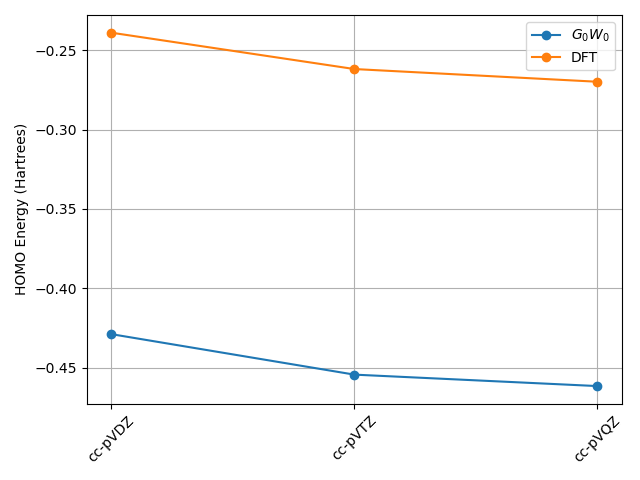
\includegraphics[width=\textwidth]{water_gw.png}
\end{figure}


\chapter{$G_0W_0$ Procedure}
\section{Iterative equation}
The procedure that was used to compute the quasiparticle energies is given by the below equation:
\begin{equation}
    \delta_{pq}F_{pq}^{HF}[\gamma^{DFT}] + \Sigma_{pp}^{corr}(\varepsilon_{p}^{QP}) = \varepsilon_{p}^{QP}
\end{equation}
We explain the notation starting from left to right. The first term corresponds to taking the diagonal $\delta_{pq}$ of the Hartree-Fock matrix $F_{pq}^{HF}$ evaluated at a given electron density $\gamma$. These electron densities are obtained from a previous mean-field calculation, either $\gamma_{DFT}$ or $\gamma_{HF}$. The second term evaluates the real part of the correlation self-energy for the $\varepsilon_{p}^{QP}$ determined in the previous iteration. The right side of the equality gives the updated quasiparticle energy.\\ The above equation is solved self-consistently. We start with an initial guess for the quasiparticle energies, which is given by the mean-field orbital energy. This is used to solve for the right-hand side quasiparticle energy of equation 2.1. In the next iteration, we use the previously obtained quasiparticle energy to formulate $\Sigma^{corr}$. This process is repeated until we reach a convergence threshold for the quasiparticle energy. We note the distinction between this and self-consistent GW (scGW); in $G_0W_0$, the iterative procedure only considers one quasiparticle energy at a time (with self-energy $\Sigma^{corr}_{pp}$), whereas scGW does not make this kind of diagonal approximation for the self-energy.
\subsection{The Fock Matrix}
In the basis of atomic orbitals, this is given by:
\begin{equation}
F_{\mu\nu}^{HF} = h_{\mu\nu} + \sum_{\lambda\sigma}P_{\lambda\sigma}(\mu\nu|\lambda\sigma) - \frac{1}{2}\sum_{\lambda\sigma}P_{\lambda\sigma}(\mu\lambda|\nu\sigma)
\end{equation}
where $h_{\mu\nu}$ is the one-electron part of the Hamiltonian, $P_{\lambda\sigma}$ is the density matrix, and $(\mu\nu|\lambda\sigma)$ is one of the two-electron integrals. \autocite{szabo_modern_2012} This is the simple form of the Hartree-Fock matrix that we want to use here and not the DFT Fock matrix. We transform this Fock matrix into the MO basis with:
\begin{equation}
   F_{pq} = \sum_{\mu} \sum_{\nu} C_{\mu p}^{*}F_{\mu\nu}C_{\nu q}
\end{equation}
where $C$ is the matrix of MO coefficients. Another useful identity is for the density matrix in terms of the MO coefficients from the mean-field calculation: 
\begin{equation}
P_{\mu\nu} = 2\sum_{i=1}^{N/2}C_{\mu i}C_{\nu i}^{*}
\end{equation}
We note that the sum runs only over the $N/2$ occupied \emph{spatial} orbitals.
\subsection{Real Correlation-Self Energy}
This is the second term in the iterative equation. It is dynamic, as opposed to the previous Fock term that was discussed, as it is updated with a new quasiparticle energy in each iteration. In the case of the $G_0W_0$ approximation, we are only interested in the diagonal element of $\Sigma^{corr}$ corresponding to the orbital with index $p$. This function is evaluated at the QP energy $\varepsilon_{p}^{QP}$ just obtained in the previous iteration. We will go into greater detail about the form of $\Sigma^{corr}$ in the next chapter.
\subsection{Quasiparticle Energy}
This is the right side, or the solution, of this equation.
\newpage
\subsection{Graphical solution}
I have been working with the HOMO of the water molecule with HF@PBE as my mean field object. I have plotted my self-energy computed for a wide range of frequencies. The line at $\omega - \varepsilon^{HF}$ should intersect with my self-energy at the same quasiparticle energy that I get from my iterative procedure, and indeed this is the case.
\begin{figure}[h]
    \centering
    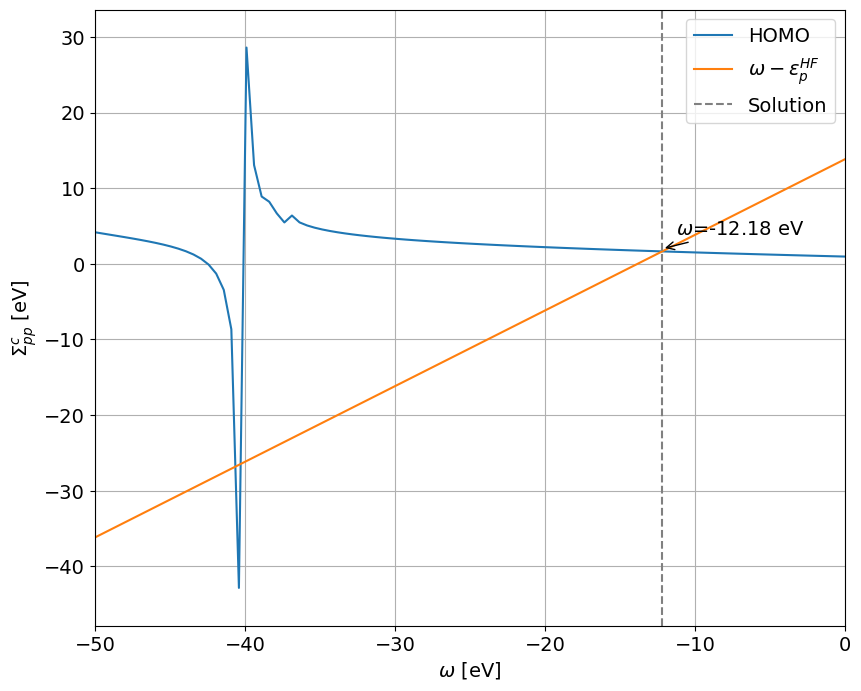
\includegraphics[width=\textwidth]{correlation_energies.png}
\end{figure}
Also, at around $\omega$ = -40 eV, one can observe a pole structure. This is a derivate discontinuity in my self-energy that would pose problems for my iterative procedure if the quasiparticle energy of the orbital that I was looking for was close to this value.


\section{Real correlation Self-Energy}
\begin{equation}
    \Sigma_{pp}^{\text{corr}}(\omega) = \sum_{\mu }^{\text{TD-DFT}}\left(\sum_{i}^{\text{occupied}} \frac{V_{pi}^{\mu }V_{ip}^{\mu }}{\omega -(\varepsilon _{i}-\Omega  _{\mu })}+ \sum_{a}^{\text{virtual}} \frac{V_{pa}^{\mu }V_{ap}^{\mu }}{\omega -(\varepsilon _{a}+\Omega  _{\mu })}\right)
\end{equation}
I have implemented the diagonal of the real part of the correlation self-energy. The $V^{\mu}$ and $\Omega_{\mu}$ are the excitation vectors and energies, respectively, from a previous TD-DFT routine; the direct Tamm-Dancoff approximation (dTDA) and the direct Random Phase Approximation (dRPA) were used here. $\omega$ is my input frequency and the $\varepsilon$ are the orbital energies from my previous mean-field calculation.



\section{Time dependent DFT}
\subsection{Random Phase Approximation}
The RPA is a linear response theory that is used to compute the excitation energies and vectors. The working matrix equation is given by \autocite{dreuw_single-reference_2005}:
\begin{equation}
\begin{bmatrix}
A & B \\
-B & -A
\end{bmatrix}
\begin{bmatrix}
X \\
Y
\end{bmatrix}
= \omega
\begin{bmatrix}
1 & 0 \\
0 & -1
\end{bmatrix}
\begin{bmatrix}
X \\
Y
\end{bmatrix}
\end{equation}
where $A$ is
\begin{equation}
    \textbf{A}_{ia,jb}=\delta _{ij} \delta _{ab} \left(\varepsilon _{a}-\varepsilon _{i}\right) + (\underline{ia}||\underline{jb})
\end{equation}
and $B$ is
\begin{equation}
    \textbf{B}_{ia,jb}=(\underline{ia}||\underline{jb})
\end{equation}
$\omega $ is a matrix with the excitation energy eigenvalues $\Omega_{\mu}$ on the diagonal. After performing the spin integration in the restricted Hartree-Fock formalism:
\begin{equation}
    (\underline{ia}||\underline{jb}) = \sum_{\alpha ,\beta } (ia||jb) = 2(ia||jb)
\end{equation}
we get for $\textbf{A}$ and $\textbf{B}$:
\begin{equation}
    \textbf{A}_{ia,jb} = \delta _{ij}\delta _{ab}(\varepsilon _{a}- \varepsilon _{i}) + 2(ia||jb)
\end{equation}
\begin{equation}
    \textbf{B}_{ia,jb} = 2(ia||jb)
\end{equation}

The excitation vectors $\textbf{V}^{\mu}$ are taken by considering a contraction of two tensors. First, we consider the sum of $\textbf{X}$ and $\textbf{Y}$ at the same excitation energy $\mu$: $\textbf{Z}_{i,a,\mu} = \textbf{X}_{i,a,\mu} + \textbf{Y}_{i,a,\mu}$. Then we contract this with the two-electron integrals:
\begin{equation}
    \textbf{W}_{p,q,i,a} = \sum_{\underline{p,q,i,a}} (\underline{pq}|\underline{ia}) = \sqrt{2} \sum_{p,q,i,a} (pq|ia)
\end{equation}
We defined a combined occupied-virtual index $\nu$, so: $\textbf{Z}_{i,a,\mu} \rightarrow \textbf{Z}_{\nu, \mu}$ and $\textbf{W}_{p,q,i,a}\rightarrow \textbf{W}_{p,q,\nu}$.\\
I probably want to carry out the deviation for this factor of $\sqrt{2}$ which was something like the following. Have I set this up correctly?
\subsubsection{Spin integration}
$\ket{\Phi  _i^a}$ has the CSF
\begin{equation}
    \ket{\Phi  _{singlet}} = \frac{1}{\sqrt{2}}(\ket{\Phi _{i\alpha }^{a\alpha  }} + \ket{\Phi _{i\beta }^{a\beta  }})
\end{equation}
We want to consider something like:
\begin{equation}
\bra{\Phi _0}
    \frac{1}{4}\sum_{pqrs} V_{pq\underline{rs}}a^{\dag}_{p}a^{\dag}_{q}a_{s}a_{r}\frac{1}{\sqrt{2}}(a^{\dag \alpha }_{a}a^{\alpha }_{i} + a^{\dag \beta }_{a}a^{\beta }_{i})\ket{\Phi _0}
\end{equation}
Consolidating constants out front and distributing the CSF terms:
\begin{equation}
    \frac{1}{4\sqrt{2}}V_{pq\underline{rs}}\bra{\Phi _0}a^{\dag}_{p}a^{\dag}_{q}a_{s}a_{r}a^{\dag \alpha }_{a}a^{\alpha }_{i}\ket{\Phi _0} + \frac{1}{4\sqrt{2}}V_{pq\underline{rs}}\bra{\Phi _0}a^{\dag}_{p}a^{\dag}_{q}a_{s}a_{r}a^{\dag \beta }_{a}a^{\beta }_{i}\ket{\Phi _0}
\end{equation}

% Inline Python code in the document
And then we form the excitation vector from:
\begin{equation}
    \textbf{V}_{pq}^{\mu} = \sum_{\nu} \textbf{W}_{p,q,\nu}\textbf{Z}_{\nu, \mu}
\end{equation}

\subsection{Tamm-Dancoff Approximation}
In this method, we neglect the $\textbf{B}$ matrix of the RPA equation. So the eigenvalue equation becomes
\begin{equation}
    \textbf{A}\textbf{X} = \omega \textbf{X}
\end{equation}
where we still have:
\begin{equation}
    \textbf{A}_{ia,jb} = \delta _{ij}\delta _{ab}(\varepsilon _{a}- \varepsilon _{i}) + 2(ia||jb)
\end{equation}
And then we follow the same procedure as in the RPA to get $\textbf{V}_{pq}^{\mu}$, where now we have $\textbf{Z}_{\nu, \mu} = \textbf{X}_{\nu, \mu}$.
\subsection{Direct approximation}
Everywhere in this code, we were considering the direct approximation, which just means that all instances of anti-symmetrized two-electron integrals are replaced by their non-symmetrized counterparts (i.e. containing just the Coulomb part with $(ia||jb) \rightarrow (ia|jb)$).
\chapter{Linearized $G_0W_0$ Density Matrix}
\subsection{Implementation}
I was able to implement these working equations. \autocite{bruneval_assessment_2019} First, we consider the fully occupied block for a certain spin:
\begin{equation}
D_{i j \sigma}^{G W}=\delta_{i j}-\sum_{\omega s} \frac{w_{i a \sigma}^s w_{j \omega \sigma}^s}{\left(\epsilon_{i \sigma}-\epsilon_{a \sigma}-\Omega_s\right)\left(\epsilon_{j o}-\epsilon_{a \sigma}-\Omega_s\right)}
\end{equation}
where the $\Omega_s$ are the excitation energies and the $w_{ij}^s$ are the excitation vectors for a single spin $\sigma$. The sum runs over all virtual orbitals and all excitation energies. The $\epsilon$ are the orbital energies from the mean-field calculation. Next, we have the virtual-virtual block:
\begin{equation}
D_{a b \sigma}^{G W}=-\sum_{i s} \frac{w_{a i \sigma}^s w_{b i \sigma}^s}{\left(\epsilon_{i \sigma}-\epsilon_{i \sigma \sigma}-\Omega_s\right)\left(\epsilon_{i \sigma}-\epsilon_{b \sigma}-\Omega_s\right)}
\end{equation}
Finally, we have the mixed block:
\begin{equation}
    D_{i b \sigma}^{G W}=\frac{1}{\epsilon_{i \sigma}-\epsilon_{b \sigma}}\left[ \sum_{as} \frac{w_{i a \sigma}^s w_{b a \sigma}^s}{\left(\epsilon_{i \sigma}-\epsilon_{a \sigma}-\Omega_s\right)} - \sum_{js} \frac{w_{i j \sigma}^s w_{b j \sigma}^s}{\left( \epsilon_{j \sigma}-\epsilon_{b \sigma}-\Omega_s\right)}\right]
\end{equation}
This all contributes to the form of the density matrix as:
\begin{equation}
    2\begin{pmatrix}
        D_{i j \sigma}^{G W} & D_{i b \sigma}^{G W} \\
        D_{bi \sigma}^{G W } & D_{a b \sigma}^{G W}
    \end{pmatrix}
\end{equation}
Where $D_{bi \sigma}^{\text{GW}}$ is simply the transpose of $D_{ib \sigma}^{\text{GW}}$, since all elements of this matrix are real. Therefore, this density matrix is Hermitian. The formulas given are only for a certain spin $\sigma$. So after we sum over both possible spins, we get the factor of 2.
\newpage
\subsection{Plotting natural occupations}
The natural occupations can be found by the diagonalizing the density matrix. They can be interpreted as being the amount of electrons in a given orbital.\autocite{szabo_modern_2012} Here we considered the one-electron density matrix from multiple methods; We started with Hartree-Fock, which contains no correlation, then we considered our implementation of the direct Random Phase Approximation (dRPA) and the direct Tamm-Dancoff Approximation (dTDA). Finally, we considered Full Configuration Interaction (FCI) as a reference, as it contains the exact correlation.
\begin{figure}[h]
    \centering
    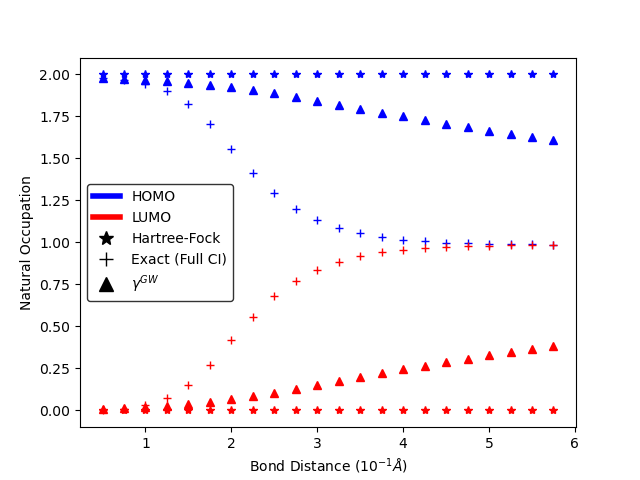
\includegraphics[width=0.8\textwidth]{h2_occupations.png}
\end{figure}
It should be noted that we considered natural occupations of the HOMO (State 1) and LUMO (State 2) of $H_2$, which has the simple MO diagram.
\begin{figure}[h]
    \centering
    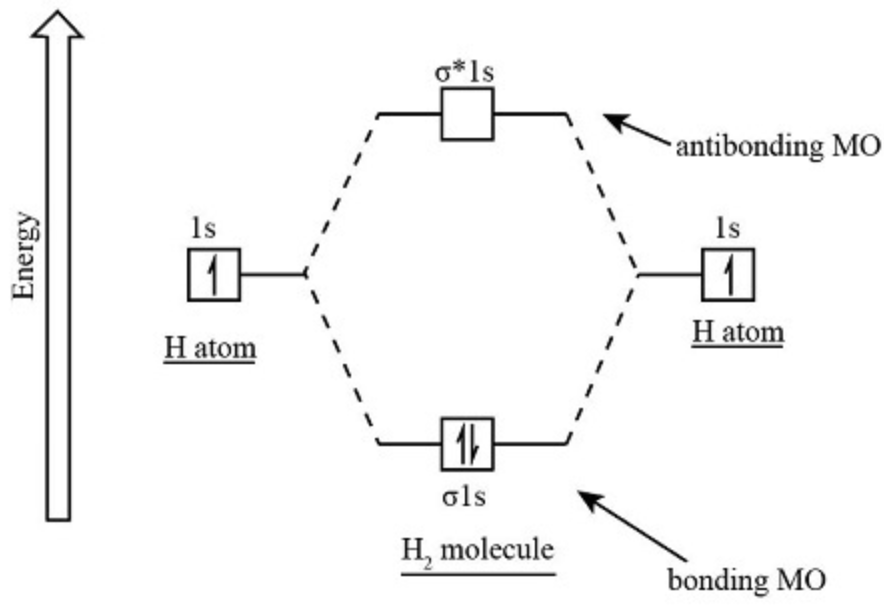
\includegraphics[width=0.5\textwidth]{h2_mo.png}
\end{figure}


\chapter{This is the Sixth Chapter}
\chapter{This is the Seventh Chapter}
\chapter{This is the Eighth Chapter}

\printbibliography[heading=bibintoc]

\appendix

\chapter{Questionnaire}
\chapter{Consent Form}

\printindex

\theendnotes

%% Pocket materials at the VERY END of thesis
\pocketmaterial
\extrachapter{Pocket Material: Map of Case Study Solar Systems} 


\end{document}
